% =========================================================================
% AAT — Figure: Bathtub Scaffold (Persistence as Contraction-Over-Drift)
% Companion to: AAT preamble, #result-persistence-condition,
%               #disc-stability-certificate
%
% Build:  pdflatex bathtub-scaffold.tex
%
% Three-rung CRA ladder: concrete (literal water vocabulary) -> metaphor
% (plain-English AAT vocabulary) -> abstract (formal AAT symbols). The
% same picture is drawn three times with different labels in identical
% spatial positions, so the analogy is visually one-to-one.
% =========================================================================
\documentclass[border=10pt]{standalone}
\usepackage{tikz}
\usepackage{amsmath,amssymb}
\usetikzlibrary{arrows.meta,decorations.pathmorphing,calc,positioning}

\begin{document}
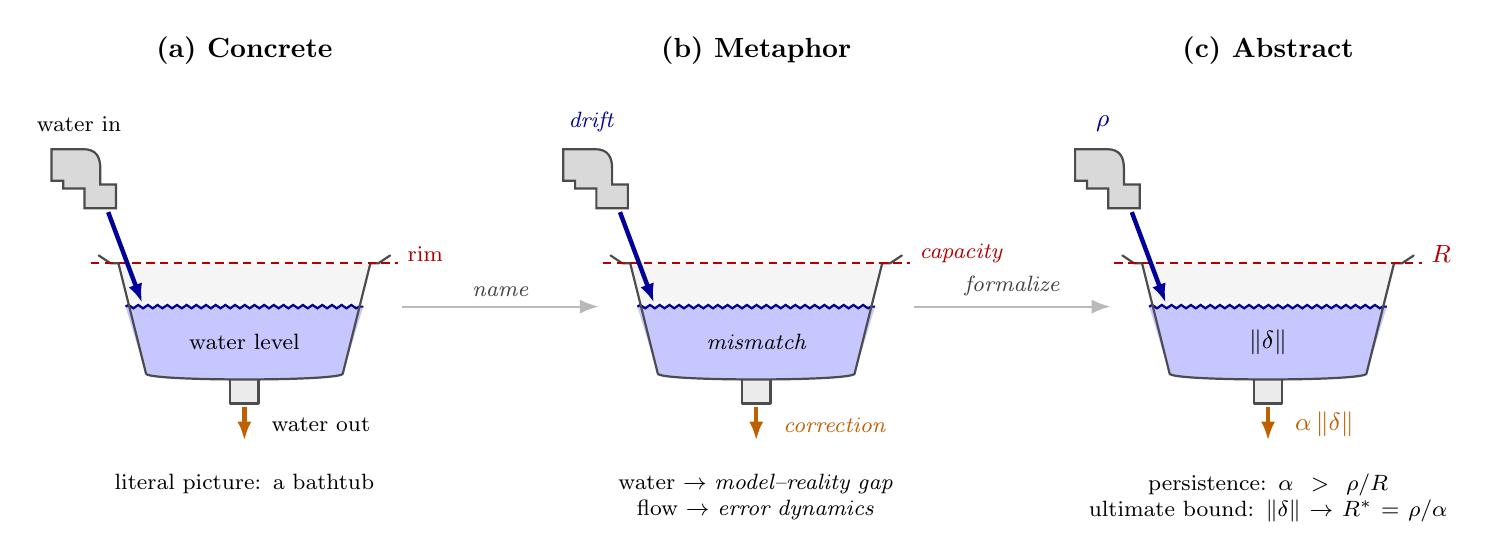
\begin{tikzpicture}[
    font=\small,
    >=Latex,
    tub/.style          = {thick, draw=black!70, line cap=round, line join=round},
    tubfill/.style      = {fill=black!4},
    water/.style        = {fill=blue!22},
    waterline/.style    = {draw=blue!55!black, thick,
                           decoration={snake, amplitude=0.6pt, segment length=3.5pt},
                           decorate},
    faucet/.style       = {thick, draw=black!70, fill=black!12, line cap=round},
    flow-in/.style      = {-{Latex[length=2.4mm]}, ultra thick, blue!60!black},
    flow-out/.style     = {-{Latex[length=2.4mm]}, ultra thick, orange!75!black},
    rimline/.style      = {densely dashed, red!70!black, thick},
    paneltitle/.style   = {font=\bfseries, anchor=south},
    panelcaption/.style = {font=\footnotesize, align=center, anchor=north,
                          text width=4.4cm},
    concrete-lbl/.style = {font=\footnotesize, align=center},
    metaphor-lbl/.style = {font=\footnotesize\itshape, align=center},
    abstract-lbl/.style = {font=\small},
    rung-arrow/.style   = {-{Latex[length=2.4mm]}, thick, gray!55}
  ]

% =========================================================
% Reusable bathtub drawing (relative to scope origin).
% Geometry:
%   inner top-left:     (-1.6, 0)        inner bottom-left:  (-1.25,-1.4)
%   inner top-right:    ( 1.6, 0)        inner bottom-right: ( 1.25,-1.4)
%   water surface y:    -0.55
%   rim line y:         0
% =========================================================
\newcommand{\drawbathtub}{%
  \fill[tubfill]
    (-1.6,0) -- (-1.25,-1.4) .. controls (-1.25,-1.5) and (1.25,-1.5) ..
    (1.25,-1.4) -- (1.6,0);
  \fill[water]
    (-1.51,-0.55) -- (-1.25,-1.4) .. controls (-1.25,-1.5) and (1.25,-1.5) ..
    (1.25,-1.4) -- (1.51,-0.55) -- cycle;
  \draw[waterline] (-1.51,-0.55) -- (1.51,-0.55);
  \draw[tub]
    (-1.85, 0.10) -- (-1.7, 0) -- (-1.6, 0) -- (-1.25,-1.4)
    .. controls (-1.25,-1.5) and (1.25,-1.5) ..
    (1.25,-1.4) -- (1.6, 0) -- (1.7, 0) -- (1.85, 0.10);
  \draw[rimline] (-1.95, 0) -- (1.95, 0);
  \draw[faucet, fill=black!15]
    (-2.45, 1.05) -- (-2.45, 1.45) -- (-2.05, 1.45)
    .. controls (-1.88, 1.45) and (-1.83, 1.35) ..
    (-1.83, 1.20) -- (-1.83, 1.00) -- (-1.63, 1.00) -- (-1.63, 0.70)
    -- (-2.03, 0.70) -- (-2.03, 0.95) -- (-2.30, 0.95) -- (-2.30, 1.05) -- cycle;
  \draw[flow-in] (-1.73, 0.65) -- (-1.30, -0.50);
  \draw[tub, fill=black!8]
    (-0.18,-1.49) -- (-0.18,-1.78) -- (0.18,-1.78) -- (0.18,-1.49);
  \draw[flow-out] (0, -1.82) -- (0, -2.25);
}

% Panel positions
\def\panelA{0}
\def\panelB{6.5}
\def\panelC{13.0}

% =========================================================
% PANEL (a) -- Concrete (literal water vocabulary)
% =========================================================
\begin{scope}[xshift=\panelA cm]
  \drawbathtub

  % Concrete labels (placed inside or just outside the bathtub region)
  \node[concrete-lbl, anchor=south] at (-2.10, 1.55) {water in};
  \node[concrete-lbl, anchor=west]  at (0.22, -2.05) {water out};
  \node[concrete-lbl]               at (0, -1.0) {water level};
  \node[concrete-lbl, anchor=west, red!70!black] at (1.95, 0.12) {rim};

  % Title and caption
  \node[paneltitle] at (0, 2.4) {(a) Concrete};
  \node[panelcaption] at (0, -2.55) {literal picture: a bathtub};
\end{scope}

% =========================================================
% PANEL (b) -- Metaphor (plain-English AAT vocabulary)
% =========================================================
\begin{scope}[xshift=\panelB cm]
  \drawbathtub

  % Metaphor labels (same positions as concrete; AAT concepts named in words)
  \node[metaphor-lbl, anchor=south, blue!60!black] at (-2.10, 1.55) {drift};
  \node[metaphor-lbl, anchor=west, orange!75!black] at (0.22, -2.05) {correction};
  \node[metaphor-lbl] at (0, -1.0) {mismatch};
  \node[metaphor-lbl, anchor=west, red!70!black] at (1.95, 0.12) {capacity};

  \node[paneltitle] at (0, 2.4) {(b) Metaphor};
  \node[panelcaption] at (0, -2.55)
    {water $\to$ \emph{model--reality gap}\\ flow $\to$ \emph{error dynamics}};
\end{scope}

% =========================================================
% PANEL (c) -- Abstract (formal AAT symbols)
% =========================================================
\begin{scope}[xshift=\panelC cm]
  \drawbathtub

  % Abstract labels (same positions; formal symbols)
  \node[abstract-lbl, anchor=south, blue!60!black] at (-2.10, 1.55) {$\rho$};
  \node[abstract-lbl, anchor=west, orange!75!black] at (0.22, -2.05)
    {$\alpha\,\lVert\delta\rVert$};
  \node[abstract-lbl] at (0, -1.0) {$\lVert\delta\rVert$};
  \node[abstract-lbl, anchor=west, red!70!black] at (1.95, 0.12) {$R$};

  \node[paneltitle] at (0, 2.4) {(c) Abstract};
  \node[panelcaption, text width=5.0cm] at (0, -2.55)
    {persistence: $\alpha > \rho/R$\\
     ultimate bound: $\lVert\delta\rVert \to R^{\ast} = \rho/\alpha$};
\end{scope}

% =========================================================
% Rung arrows between panels (signaling the CRA progression)
% =========================================================
\draw[rung-arrow] (2.0, -0.55) -- (4.5, -0.55)
  node[midway, above, font=\footnotesize\itshape, gray!50!black] {name};
\draw[rung-arrow] (8.5, -0.55) -- (11.0, -0.55)
  node[midway, above, font=\footnotesize\itshape, gray!50!black] {formalize};

\end{tikzpicture}
\end{document}
